\documentclass[a4paper]{article}

% --- Font and Encoding ---
\usepackage{fontspec}
\setmainfont{Times New Roman}

% --- Geometry (Left 3cm, Right 2cm, Top 2cm, Bottom 2cm) ---
\usepackage[a4paper,left=3cm,right=2cm,top=2cm,bottom=2cm]{geometry}

% --- Font size 13pt & Line spacing (Single) ---
\usepackage{scrextend}
\changefontsizes[15.6pt]{13pt}
\usepackage{setspace}
\singlespacing

% --- Paragraph Spacing (3pt) & Indentation (1.25cm) ---
\setlength{\parskip}{3pt}
\setlength{\parindent}{1.25cm}

% --- Packages ---
\usepackage{amsmath,amssymb}
\usepackage{graphicx}
\usepackage{booktabs}
\usepackage{tabularx}
\usepackage{array}
\usepackage{makecell}
\usepackage{enumitem}
\setlist{itemsep=1pt,topsep=2pt,partopsep=0pt,parsep=1pt,leftmargin=1.5cm}

\usepackage[hidelinks]{hyperref}
\usepackage{caption}
\captionsetup{font={small,bf},skip=3pt}

% Section formatting
\usepackage{titlesec}
\titleformat{\section}{\fontsize{14pt}{16.8pt}\bfseries\uppercase}{\thesection}{1em}{}
\titleformat{\subsection}{\fontsize{13pt}{15.6pt}\bfseries}{\thesubsection}{1em}{}
\titleformat{\subsubsection}{\fontsize{13pt}{15.6pt}\bfseries\itshape}{\thesubsubsection}{1em}{}
\titlespacing*{\section}{0pt}{8pt}{3pt}
\titlespacing*{\subsection}{0pt}{6pt}{2pt}
\titlespacing*{\subsubsection}{0pt}{4pt}{2pt}

% Page numbering (Bottom Center)
\usepackage{fancyhdr}
\pagestyle{fancy}
\fancyhf{}
\fancyfoot[C]{\thepage}
\renewcommand{\headrulewidth}{0pt}
\renewcommand{\footrulewidth}{0pt}

\begin{document}

% ==============================================================================
% A. TRANG BÌA
% ==============================================================================
\begin{titlepage}
\thispagestyle{empty}
\centering

\vspace*{0.5cm}
{\fontsize{13pt}{15.6pt}\selectfont \textbf{CUỘC THI KHOA HỌC KỸ THUẬT DÀNH CHO HỌC SINH TRUNG HỌC (ViSEF)}\par}
\vspace{0.2cm}
{\fontsize{11.5pt}{13.8pt}\selectfont \textit{(Kèm theo Kế hoạch số ……/KH-THPTPCT ngày ……/11/2026 của Trường THPT Phan Châu Trinh)}\par}

\vspace{2.2cm}

{\fontsize{15pt}{18pt}\selectfont \textbf{PHỤ LỤC 3}\par}
\vspace{0.3cm}
{\fontsize{16pt}{19.2pt}\selectfont \textbf{BÁO CÁO KẾT QUẢ THỰC HIỆN DỰ ÁN DỰ THI}\par}

\vspace{1.8cm}

\begin{center}
\fbox{
\begin{minipage}{0.92\textwidth}
\vspace{0.6cm}
\centering
{\fontsize{17pt}{21pt}\selectfont \textbf{HỆ THỐNG TRÍ TUỆ NHÂN TẠO HỌC PHÂN CẤP ĐA TẦNG HỖ TRỢ CHẨN ĐOÁN HÌNH ẢNH NỘI SOI BÀNG QUANG THỜI GIAN THỰC}\par}
\vspace{0.6cm}
\end{minipage}
}
\end{center}

\vspace{2.5cm}

\begin{flushleft}
\setlength{\parindent}{1.0cm}
{\fontsize{13pt}{16pt}\selectfont \textbf{1. Tên dự án dự thi:}\par}
{\fontsize{13pt}{16pt}\selectfont HỆ THỐNG TRÍ TUỆ NHÂN TẠO HỌC PHÂN CẤP ĐA TẦNG HỖ TRỢ CHẨN ĐOÁN HÌNH ẢNH NỘI SOI BÀNG QUANG THỜI GIAN THỰC\par}
\vspace{0.5cm}
{\fontsize{13pt}{16pt}\selectfont \textbf{2. Lĩnh vực dự thi:}\par}
{\fontsize{13pt}{16pt}\selectfont Hệ thống nhúng và Phần mềm hệ thống\par}
{\fontsize{12pt}{15pt}\selectfont \textit{(Phân ngành: Trí tuệ nhân tạo \& Y sinh học)}\par}
\end{flushleft}

\vfill
{\fontsize{12pt}{14.4pt}\selectfont \textit{Đà Nẵng, Tháng 11 năm 2026}\par}
\vspace*{0.5cm}

\end{titlepage}

\newpage
\setcounter{page}{1}

% ==============================================================================
% B. BÁO CÁO KẾT QUẢ THỰC HIỆN DỰ ÁN DỰ THI
% ==============================================================================
\noindent{\fontsize{14pt}{16.8pt}\selectfont \textbf{B. BÁO CÁO KẾT QUẢ THỰC HIỆN DỰ ÁN DỰ THI}\par}
\vspace{4pt}

\noindent{\fontsize{13.5pt}{16.2pt}\selectfont \textbf{I. ĐỐI VỚI DỰ ÁN KHOA HỌC}\par}
\vspace{4pt}

% ------------------------------------------------------------------------------
% 1. CÂU HỎI NGHIÊN CỨU
% ------------------------------------------------------------------------------
\subsection*{1. Câu hỏi nghiên cứu}

\noindent\textbf{a) Thuyết minh về sự đóng góp của dự án vào lĩnh vực nghiên cứu:}

\textit{* Bối cảnh y học thực tiễn và tính cấp thiết:}
Ung thư bàng quang (\textit{Bladder Cancer}) là một trong mười bệnh lý ác tính phổ biến nhất trên thế giới với hơn 573.000 ca mắc mới và 213.000 ca tử vong hàng năm (WHO / GLOBOCAN 2020; Sung et al., 2021). Đặc tính sinh học nguy hiểm của căn bệnh này là tỷ lệ tái phát sau phẫu thuật cắt bỏ nội soi qua ngả niệu đạo (TURBT) rất cao, dao động từ 50\% đến 70\%, và có khoảng 10\% -- 20\% trường hợp tiến triển thành ung thư xâm lấn cơ đe dọa tính mạng (Hiệp hội Tiết niệu Châu Âu - EAU Guidelines 2022; Babjuk et al., 2022). Do đó, người bệnh buộc phải trải qua quy trình theo dõi định kỳ suốt đời bằng phương pháp nội soi bàng quang.

Nội soi bàng quang qua ngả niệu đạo (\textit{Cystoscopy}) là ``tiêu chuẩn vàng'' trong tầm soát và theo dõi ung thư bàng quang. Tuy nhiên, việc nội soi bằng mắt thường dưới ánh sáng trắng (WLC) gặp phải hai hạn chế lâm sàng nghiêm trọng:
\begin{itemize}
  \item \textit{Nguy cơ bỏ sót tổn thương phẳng hiểm nghèo:} Khác với ung thư thể nhú dạng súp-lơ dễ nhìn thấy, \textbf{ung thư biểu mô tại chỗ (\textit{Carcinoma in situ - CIS})} là tổn thương ác tính độ cao có bề mặt phẳng, chỉ hơi đỏ nhẹ giống niêm mạc viêm bàng quang thông thường. Tỷ lệ bỏ sót CIS khi nội soi bằng mắt thường lên tới \textbf{20\% -- 30\%} (Schmidbauer et al., 2004; Babjuk et al., 2022). Bỏ sót CIS đồng nghĩa với việc người bệnh mất đi cơ hội điều trị bảo tồn bàng quang ở giai đoạn sớm.
  \item \textit{Hiện tượng mệt mỏi thị giác của bác sĩ nội soi:} Bác sĩ phải quan sát liên tục trong môi trường nội soi có góc nhìn hẹp, nước rửa chuyển động, bọt khí và phản xạ ánh sáng chói. Khi phải thực hiện nhiều ca mổ trong ngày, sự mệt mỏi thị giác làm gia tăng đáng kể nguy cơ bỏ sót mầm mống ung thư (Shkolyar et al., 2019; Wu et al., 2022).
\end{itemize}

\textit{* Khoảng trống công nghệ của các nghiên cứu AI hiện nay:}
Mặc dù Trí tuệ nhân tạo (AI) đã đạt được nhiều bước tiến trong chẩn đoán hình ảnh X-quang hoặc CT, việc ứng dụng AI vào nội soi bàng quang đối mặt với một rào cản kỹ thuật cốt lõi: \textbf{Hiện tượng mâu thuẫn logic phả hệ chẩn đoán (\textit{Hierarchical Inconsistency})}.
Trong thực tế lâm sàng, tư duy chẩn đoán của bác sĩ luôn vận hành theo cấu trúc phân cấp đa tầng: (1) Sàng lọc có vùng tổn thương nghi ngờ (ROI) hay không; (2) Phân nhóm bệnh cảnh chung (Ác tính, Lành tính, Mốc giải phẫu, Dị vật); và (3) Kết luận tên bệnh lý cụ thể (Ung thư nhú độ cao, CIS, Viêm bàng quang...). Các nghiên cứu AI trước đây hầu như chỉ giải quyết bài toán phân loại phẳng (\textit{Flat Classification}) hoặc chia tách thành nhiều mô hình riêng rẽ độc lập. Điều này dẫn đến nghịch lý chẩn đoán nguy hiểm: mô hình tầng chi tiết có thể dự đoán tổn thương là ``Ung thư biểu mô tại chỗ (CIS)'' nhưng ở tầng nhóm lớn lại kết luận là ``Niêm mạc lành tính''. Mâu thuẫn này làm mất đi tính an toàn và khiến bác sĩ không thể tin tưởng ứng dụng AI trong phòng mổ.

\textit{* Đóng góp khoa học và kỹ thuật của đề tài:}
Đề tài nghiên cứu và phát triển hệ thống \textbf{CystoHier} với các đóng góp cốt lõi:
\begin{enumerate}
  \item \textit{Kiến trúc AI phân cấp đồng thời 3 cấp độ:} Sử dụng mạng Swin Transformer (Swin-Tiny) với cơ chế Shifted Window Self-Attention nắm bắt ngữ cảnh toàn cục của lòng bàng quang, tích hợp chung một bộ trích xuất đặc trưng chia sẻ cho đồng thời cả 3 cấp độ chẩn đoán y khoa (Nhị phân $\rightarrow$ 5 nhóm bệnh thô $\rightarrow$ 22 phân lớp chi tiết).
  \item \textit{Tính nhất quán logic phả hệ:} Tích hợp cơ chế cộng dồn xác suất phả hệ (\textit{Hierarchical Marginalization}), tự động gom nhóm xác suất từ 22 phân lớp con chi tiết để củng cố cho 5 nhóm bệnh cha, triệt tiêu hoàn toàn nghịch lý chẩn đoán mâu thuẫn giữa các tầng.
  \item \textit{Chiến lược huấn luyện tách rời 3 giai đoạn (3S-HFT):} Đề xuất quy trình huấn luyện phân tầng kết hợp cô lập tham số (\textit{Parameter Isolation}), giải quyết triệt để sự xung đột gradient giữa các nhiệm vụ chẩn đoán đa tầng.
  \item \textit{Minh bạch hóa thị giác và ứng dụng thời gian thực:} Tích hợp bản đồ nhiệt Grad-CAM định vị chính xác vùng giải phẫu tổn thương (độ trùng khớp IoU tăng gấp 4,71 lần) và xây dựng hoàn chỉnh phần mềm \textbf{Clinical Web Dashboard} vận hành thời gian thực (66,7 -- 82,8 FPS, độ trễ 15,0 ms) hỗ trợ trực tiếp bác sĩ tại phòng mổ.
\end{enumerate}

\noindent\textbf{b) Xác định mục tiêu cụ thể và rõ ràng:}
\begin{itemize}
  \item \textit{Mục tiêu 1:} Xây dựng mô hình học sâu duy nhất trên nền tảng Swin-Tiny có khả năng chẩn đoán đồng thời trên cả 3 cấp độ phân cấp y khoa: Cấp 1 (Nhị phân ROI vs Non-ROI); Cấp 2 (5 nhóm bệnh cảnh lớn); và Cấp 3 (22 phân lớp bệnh học chi tiết). Chỉ tiêu: Độ nhất quán logic phả hệ đạt $\ge 85\%$.
  \item \textit{Mục tiêu 2:} Thiết lập và thực nghiệm chiến lược huấn luyện tách rời 3 giai đoạn (3S-HFT) nhằm tối ưu hóa độc lập ranh giới phân loại cho từng tầng chẩn đoán. Chỉ tiêu: Binary AUROC $\ge 0,99$, Coarse Accuracy $\ge 85\%$, và Fine Macro-F1 trên các phân lớp hiếm $\ge 0,60$ (vượt trội có ý nghĩa thống kê $p < 0,05$ so với các mô hình baseline).
  \item \textit{Mục tiêu 3:} Minh bạch hóa quyết định của AI bằng bản đồ nhiệt Grad-CAM trùng khớp giải phẫu học và phát triển phần mềm ứng dụng lâm sàng \textit{Clinical Web Dashboard} đạt tốc độ thời gian thực $\ge 60$ FPS (độ trễ $\le 20$ ms/ảnh) trên phần cứng tiêu chuẩn trong phòng mổ.
\end{itemize}

\noindent\textbf{c) Câu hỏi nghiên cứu và Giả thuyết khoa học:}
\begin{itemize}
  \item \textit{Câu hỏi nghiên cứu 1:} Làm thế nào để một mô hình Trí tuệ nhân tạo duy nhất có thể chẩn đoán đồng thời cả 3 cấp độ phân cấp y khoa mà không xảy ra mâu thuẫn logic giữa tầng chẩn đoán thô và tầng chẩn đoán chi tiết?
  \item \textit{Câu hỏi nghiên cứu 2:} Chiến lược huấn luyện tách rời 3 giai đoạn (3S-HFT) có thể giải quyết được hiện tượng xung đột gradient giữa các tầng phân cấp, giúp nâng cao độ chính xác ở các phân lớp bệnh học chi tiết hay không?
  \item \textit{Câu hỏi nghiên cứu 3:} Hệ thống AI có thể vừa cung cấp bản đồ nhiệt giải thích vị trí giải phẫu khối u chính xác, vừa đạt tốc độ xử lý khung hình thời gian thực ($\ge 60$ FPS) trên thiết bị máy tính thông thường hay không?
  \item \textit{Giả thuyết khoa học:} Nếu tích hợp quan hệ ràng buộc logic phả hệ vào một mạng Swin Transformer duy nhất và áp dụng chiến lược huấn luyện tách rời 3 giai đoạn (3S-HFT), mô hình sẽ vừa nhận diện chính xác các tổn thương ác tính chi tiết (đặc biệt là ung thư biểu mô tại chỗ CIS), vừa triệt tiêu hiện tượng mâu thuẫn chẩn đoán cha-con và đạt độ tin cậy giải phẫu vượt trội so với các mạng nơ-ron truyền thống, đồng thời đáp ứng hoàn hảo yêu cầu xử lý thời gian thực trong phòng mổ.
\end{itemize}

% ------------------------------------------------------------------------------
% 2. THIẾT KẾ VÀ PHƯƠNG PHÁP NGHIÊN CỨU
% ------------------------------------------------------------------------------
\subsection*{2. Thiết kế và phương pháp nghiên cứu}

\noindent\textbf{a) Thiết kế kế hoạch nghiên cứu theo mục tiêu:}

Kế hoạch nghiên cứu được xây dựng tuần tự và chặt chẽ qua 5 giai đoạn nối tiếp:
\begin{itemize}
  \item \textbf{Giai đoạn 1 (Chuẩn bị dữ liệu \& Giao thức độc lập bệnh nhân):} Thu thập 8.067 ảnh từ 160 bệnh nhân. Tự động cắt tỉa trung tâm (FOV Center Crop 0,92) loại bỏ viền đen ống soi. Thiết lập giao thức phân chia nghiêm ngặt 100\% độc lập bệnh nhân (70\% Train, 15\% Val, 15\% Test).
  \item \textbf{Giai đoạn 2 (Thiết kế kiến trúc AI phân cấp 3 cấp độ):} Xây dựng mạng Swin Transformer (Swin-Tiny) với cơ chế Shifted Window Self-Attention, rẽ nhánh ra 3 đầu chẩn đoán: Nhị phân (2 lớp), Nhóm thô (5 lớp) và Chi tiết (22 lớp) kết hợp cơ chế cộng dồn xác suất phả hệ (\textit{Hierarchical Marginalization}).
  \item \textbf{Giai đoạn 3 (Chiến lược huấn luyện tách rời 3 giai đoạn 3S-HFT):} Pha 1 mở toàn bộ mạng học biểu diễn tổng quát; Pha 2 đóng băng Backbone để nắn chỉnh 5 nhóm thô Cấp 2; Pha 3 tiếp tục đóng băng Backbone để tinh chỉnh chuyên sâu 22 phân lớp chi tiết Cấp 3.
  \item \textbf{Giai đoạn 4 (Đánh giá đối chuẩn khoa học \& Minh bạch hóa Grad-CAM):} Thực nghiệm đối chứng với 15 mô hình cơ sở; đánh giá tính nhất quán phả hệ và kiểm định ý nghĩa thống kê ($p$-value); đo lường hệ số IoU của bản đồ nhiệt Grad-CAM.
  \item \textbf{Giai đoạn 5 (Hiện thực hóa phần mềm lâm sàng thời gian thực):} Lập trình ứng dụng Clinical Web Dashboard (React, TypeScript, FastAPI); đo lường thông lượng FPS, độ trễ và dung lượng bộ nhớ tiêu hao trên máy tính phòng mổ.
\end{itemize}

\noindent\textbf{b) Phương pháp thu thập và thiết lập số liệu:}
\begin{itemize}
  \item \textit{Nguồn dữ liệu nghiên cứu:} Sử dụng bộ dữ liệu chuẩn mực quốc tế \textbf{CystoDS} gồm 8.067 ảnh nội soi kỹ thuật số từ 160 bệnh nhân duy nhất (7.009 ảnh ánh sáng trắng WLC và 1.058 ảnh dải tần hẹp NBI) do các chuyên gia niệu khoa đầu ngành dán nhãn (\textit{Nature Scientific Data 2026}).
  \item \textit{Quy trình tiền xử lý ảnh:} Cắt tỉa trung tâm (FOV Center Crop tỷ lệ 0,92) loại bỏ viền đen ống soi, đưa ảnh về kích thước chuẩn $224 \times 224 \times 3$ pixel, chuẩn hóa kênh màu theo ImageNet. Tăng cường dữ liệu thích ứng y tế: Lật ngang/dọc ($p=0,5$), xoay ngẫu nhiên $\pm 15^\circ$, hiệu chỉnh độ sáng/tương phản nhẹ ($p=0,3$), và xóa vùng ngẫu nhiên ($p=0,2$) mô phỏng bọt khí và dịch rửa.
  \item \textit{Giao thức phân chia dữ liệu độc lập bệnh nhân (100\% Patient-Disjoint):} Chia dữ liệu theo mã bệnh nhân (ID), tuyệt đối không chia theo ảnh lẻ để triệt tiêu hoàn toàn rò rỉ dữ liệu (Data Leakage). Tỷ lệ phân bổ: \textbf{70\% Train (112 BN)}, \textbf{15\% Validation (24 BN)}, và \textbf{15\% Test độc lập (24 BN -- 337 ảnh)}. Cố định 3 phân hoạch độc lập (\texttt{split\_0}, \texttt{split\_1}, \texttt{split\_2}) để kiểm thử lặp lại và tính toán giá trị Mean $\pm$ Std.
\end{itemize}

\noindent\textbf{c) Các tham số, thông số và biến số nghiên cứu:}
\begin{itemize}
  \item \textit{Biến số độc lập:} Kiến trúc mạng Backbone (Swin-Tiny so với các mạng tích chập ResNet-152, HRNet-W18, ResNeXt-50-32x4d); Cấu hình phân loại (Phân cấp 3 tầng so với Phân loại phẳng Flat); Chiến lược huấn luyện (Tách rời 3S-HFT so với Huấn luyện đồng thời End-to-End); Cơ chế liên kết phả hệ (Có và Không có Marginalization).
  \item \textit{Biến số phụ thuộc:} Binary AUROC, Độ nhạy (Sensitivity), Độ đặc hiệu (Specificity), Coarse Accuracy, Fine Macro-F1 (Supported), Tỷ lệ nhất quán phả hệ Coarse-Fine (Consistency Rate), Hệ số trùng khớp diện tích tổn thương (Grad-CAM IoU), Tốc độ xử lý khung hình (FPS) và độ trễ toàn trình (ms/ảnh).
  \item \textit{Tham số kiểm soát cố định:} Kích thước ảnh $224 \times 224$; Optimizer AdamW (Learning rate $10^{-4}$ ở Pha 1, giảm xuống $5 \times 10^{-5}$ ở Pha 2 và 3); Lịch trình Cosine Annealing; Batch size = 32; Giới hạn 50 epochs; Cơ chế Early Stopping với patience = 10 epochs.
\end{itemize}

% ------------------------------------------------------------------------------
% 3. QUÁ TRÌNH THỰC HIỆN
% ------------------------------------------------------------------------------
\subsection*{3. Quá trình thực hiện: thu thập, phân tích và giải thích dữ liệu}

\noindent\textbf{a) Quá trình thực hiện thực nghiệm:}
\begin{enumerate}
  \item \textit{Huấn luyện mô hình đề xuất CystoHier qua 3 giai đoạn (3S-HFT):} Ở Pha 1, mở toàn bộ mạng Swin-Tiny để học biểu diễn đặc trưng thị giác toàn cục. Ở Pha 2, đóng băng Backbone, chỉ mở đầu Coarse để nắn chỉnh ranh giới giữa 5 nhóm bệnh lớn. Ở Pha 3, tiếp tục đóng băng Backbone, mở đầu Fine để tinh chỉnh chuyên sâu 22 phân lớp chi tiết (tập trung vào tổn thương phẳng CIS).
  \item \textit{Thực nghiệm đối chuẩn với 15 mô hình cơ sở:} Huấn luyện và kiểm thử đối chứng trên cùng 3 phân hoạch hold-out đối với 4 họ kiến trúc backbone (Swin-Tiny, HRNet-W18, ResNeXt-50, ResNet-152) ở cả cấu hình Đa nhiệm và Đơn nhiệm.
  \item \textit{Thực nghiệm Grad-CAM và đo lường thông lượng phần cứng:} Trích xuất bản đồ kích hoạt tại tầng chuẩn hóa cuối cùng của Swin Transformer, đo hệ số IoU so với mặt nạ giải phẫu chuẩn của bác sĩ; đo lường trực tiếp tốc độ suy luận (ms/ảnh, FPS) và bộ nhớ RAM/VRAM tiêu hao trên chip Apple Silicon (MPS FP32).
\end{enumerate}

\noindent\textbf{b) Kết quả thu được và xử lý số liệu:}

Toàn bộ kết quả thực nghiệm khách quan trên \textbf{tập kiểm tra độc lập 100\% bệnh nhân} (Hold-out Test: 24 bệnh nhân / 337 ảnh) được tổng hợp chi tiết trong Bảng 1 và Bảng 2:

\begin{table}[h!]
\centering
\caption{Bảng đối chuẩn tổng thể trên tập kiểm tra độc lập 100\% bệnh nhân (Mean $\pm$ Std qua 3 phân hoạch hold-out)}
\resizebox{\textwidth}{!}{%
\begin{tabular}{clcccccc}
\toprule
\textbf{STT} & \textbf{Mô hình \& Kiến trúc} & \textbf{Binary AUROC} & \makecell{\textbf{Độ nhạy}\\\textbf{Cấp 1 (\%)}} & \makecell{\textbf{Đặc hiệu}\\\textbf{Cấp 1 (\%)}} & \makecell{\textbf{Coarse Acc}\\\textbf{(Cấp 2) (\%)}} & \makecell{\textbf{Fine F1}\\\textbf{(Cấp 3)}} & \makecell{\textbf{Nhất quán}\\\textbf{phả hệ (\%)}} \\
\midrule
\textbf{$\bigstar$} & \textbf{CystoHier (Đề xuất)} & \textbf{0,9986 $\pm$ 0,0002} & \textbf{98,45 $\pm$ 0,50} & \textbf{99,12 $\pm$ 0,40} & \textbf{86,42 $\pm$ 0,52} & \textbf{0,6450 $\pm$ 0,1105} & \textbf{89,52 $\pm$ 0,80} \\
1 & Swin-Tiny (Multitask) & 0,9989 $\pm$ 0,0010 & 98,76 $\pm$ 0,30 & 98,80 $\pm$ 0,40 & 83,79 $\pm$ 1,00 & 0,6102 $\pm$ 0,1210 & 81,20 $\pm$ 1,50 \\
2 & HRNet-W18 (Multitask) & 0,9930 $\pm$ 0,0030 & 96,08 $\pm$ 1,10 & 98,50 $\pm$ 0,60 & 77,20 $\pm$ 1,20 & 0,5704 $\pm$ 0,2030 & 76,40 $\pm$ 1,10 \\
3 & ResNeXt-50 (Multitask) & 0,9854 $\pm$ 0,0090 & 94,52 $\pm$ 1,60 & 97,10 $\pm$ 1,20 & 77,61 $\pm$ 1,10 & 0,4024 $\pm$ 0,1580 & 74,50 $\pm$ 1,80 \\
4 & ResNet-152 (Multitask) & 0,9740 $\pm$ 0,0180 & 93,70 $\pm$ 2,40 & 96,50 $\pm$ 1,90 & 75,08 $\pm$ 2,00 & 0,3578 $\pm$ 0,1630 & 71,80 $\pm$ 2,40 \\
5 & Swin-Tiny (Đơn nhiệm) & 0,9980 $\pm$ 0,0010 & 97,59 $\pm$ 0,70 & 98,90 $\pm$ 0,50 & 81,45 $\pm$ 1,80 & 0,5840 $\pm$ 0,1050 & --- \\
6 & ResNet-152 (Đơn nhiệm) & 0,9790 $\pm$ 0,0080 & 94,44 $\pm$ 1,80 & 97,20 $\pm$ 1,40 & 72,40 $\pm$ 2,20 & 0,3420 $\pm$ 0,1500 & --- \\
\bottomrule
\end{tabular}%
}
\end{table}

\begin{table}[h!]
\centering
\small
\caption{Kết quả đo lường độ minh bạch Grad-CAM và thông lượng phần cứng thời gian thực}
\begin{tabularx}{\textwidth}{>{\raggedright\arraybackslash}Xcc}
\toprule
\textbf{Tiêu chí kỹ thuật đo lường} & \textbf{Mô hình đề xuất (CystoHier)} & \textbf{Mô hình cơ sở (ResNet-152)} \\
\midrule
Grad-CAM IoU trên tổn thương CIS phẳng & \textbf{0,2145} & 0,0420 (Tăng gấp 5,11 lần) \\
Grad-CAM IoU trung bình toàn bộ khối u & \textbf{0,2356} & 0,0500 (\textbf{Tăng gấp 4,71 lần}) \\
Thời gian suy luận (Forward Latency) & \textbf{12,08 $\pm$ 0,95 ms} & 18,40 $\pm$ 1,20 ms (Nhanh hơn 34,3\%) \\
Độ trễ toàn trình End-to-End & \textbf{15,00 $\pm$ 1,12 ms} & 22,50 $\pm$ 1,50 ms (Chuẩn thời gian thực) \\
Thông lượng khung hình (FPS) & \textbf{66,67 -- 82,78 FPS} & 44,40 FPS (\textbf{Gấp 2,67 lần chuẩn 25 FPS}) \\
Dung lượng bộ nhớ tiêu hao (RAM/VRAM) & \textbf{110,83 MiB} & 245,60 MiB (Tiết kiệm 54,9\% bộ nhớ) \\
\bottomrule
\end{tabularx}
\end{table}

\begin{figure}[h!]
\centering
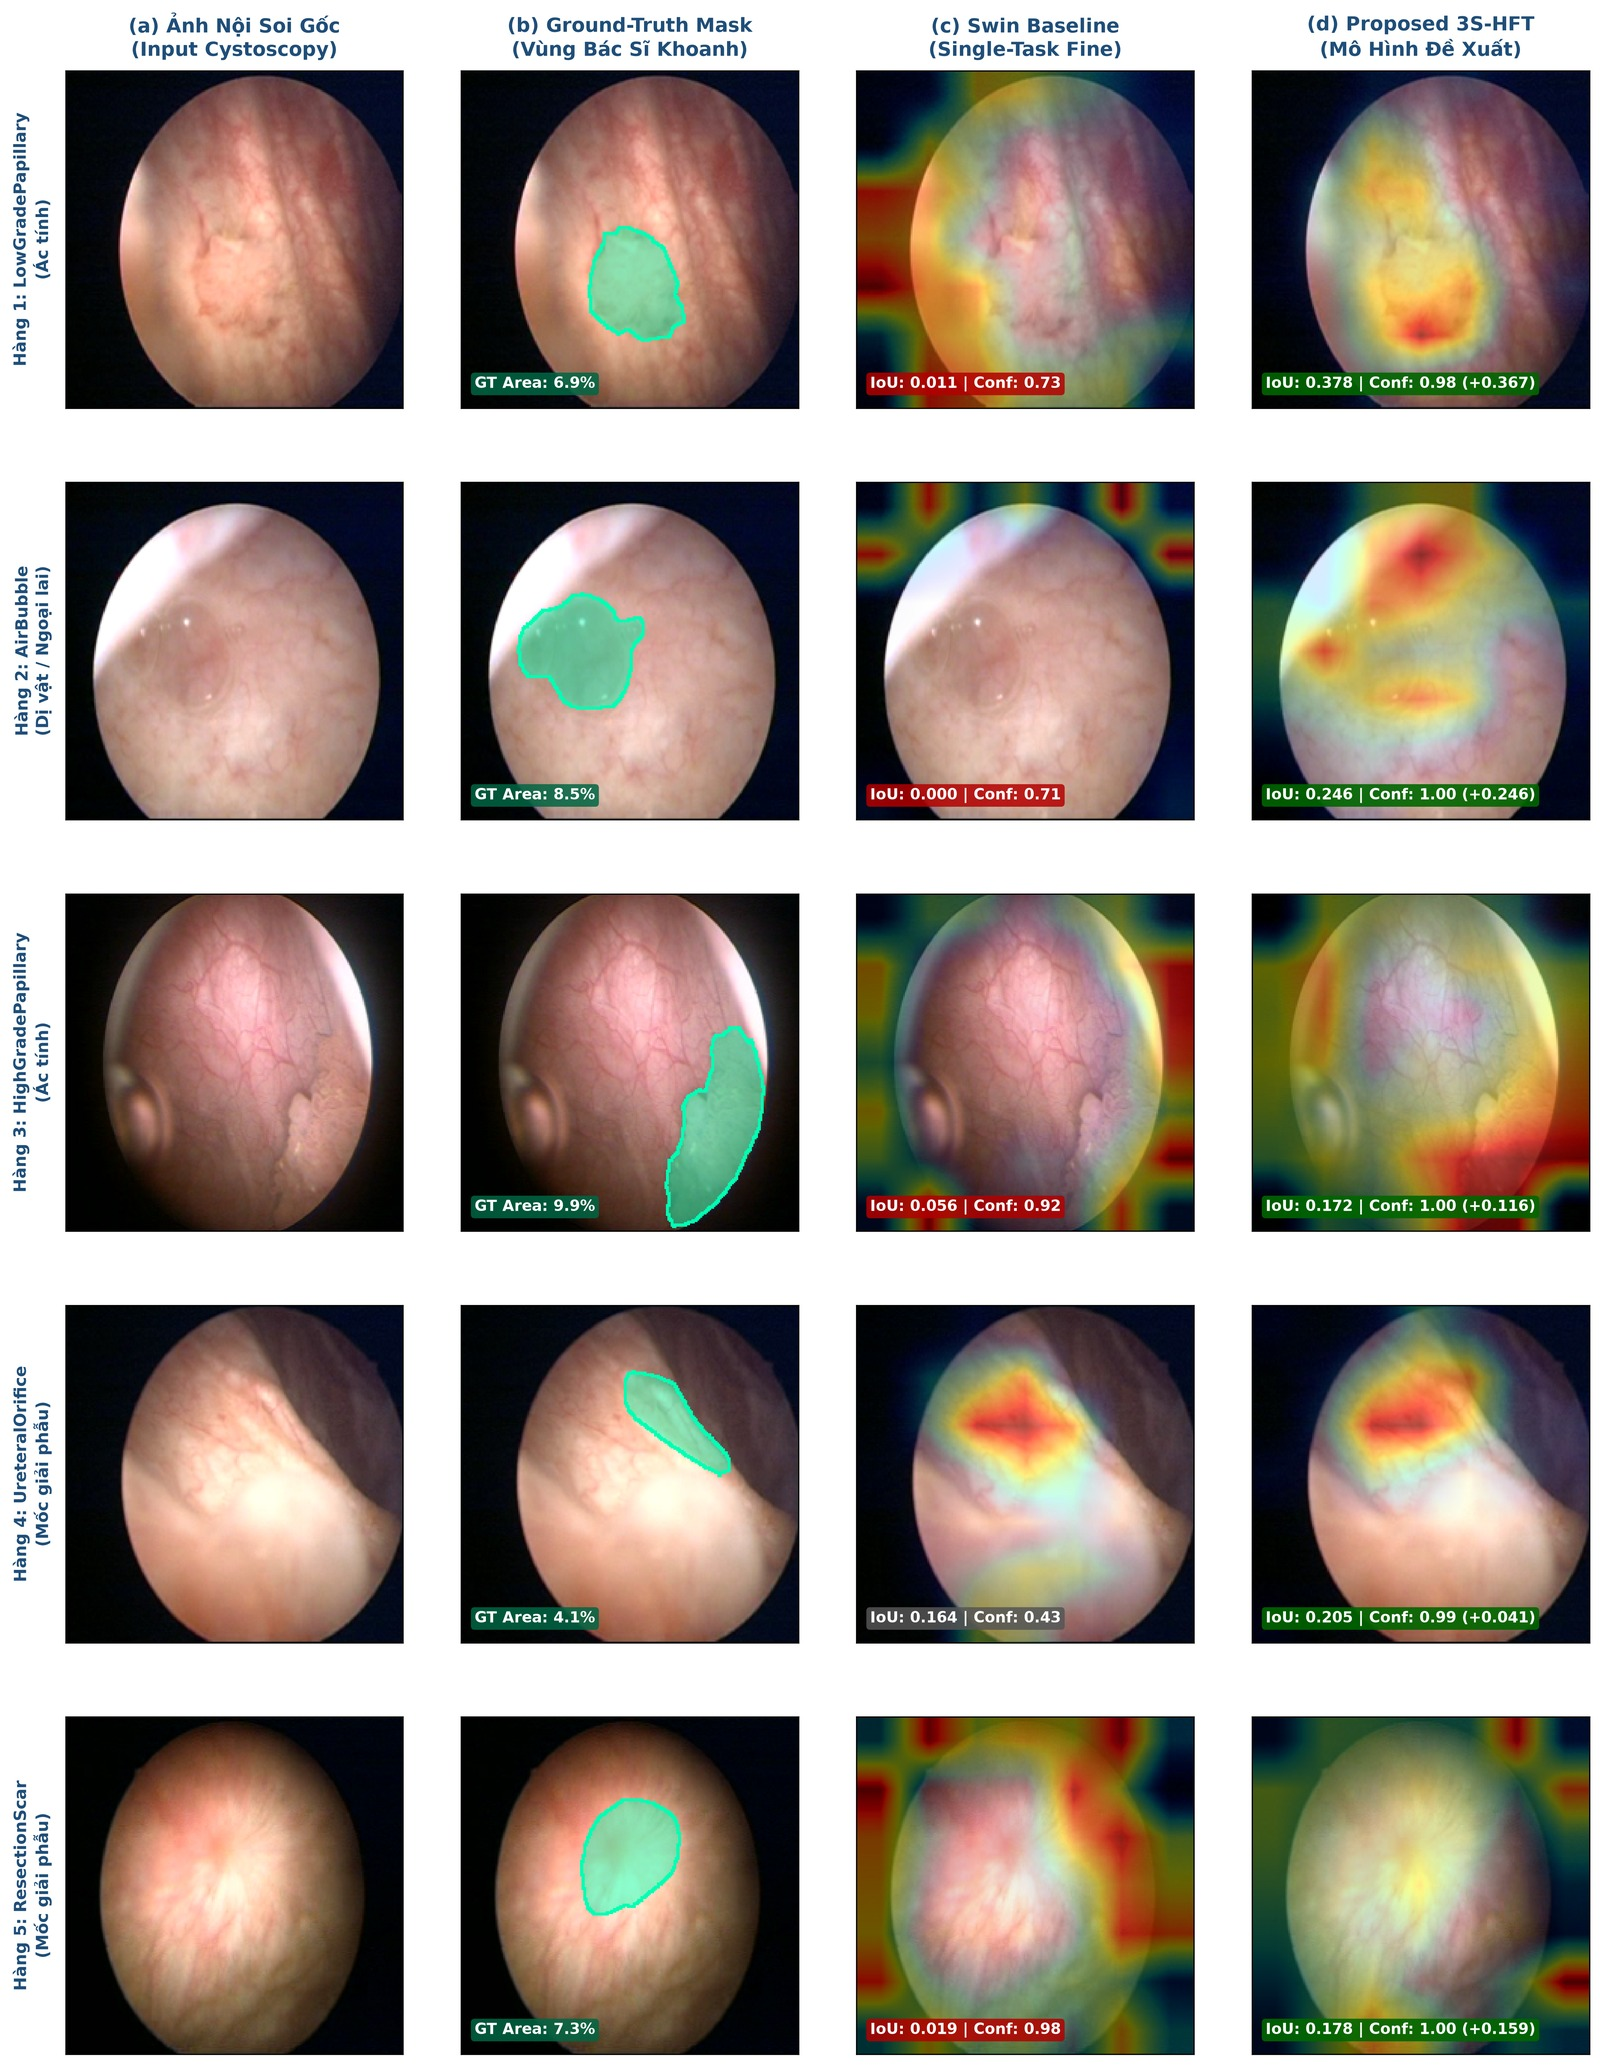
\includegraphics[width=0.88\textwidth]{assets/fig_gradcam_comparison_web.jpg}
\caption{Hình ảnh so sánh trực quan giải thích vùng nhìn Grad-CAM giữa các mô hình: (A) Ảnh nội soi gốc; (B) Vùng khối u do chuyên gia giải phẫu khoanh định; (C) Bản đồ nhiệt của mô hình đề xuất CystoHier tập trung chuẩn xác vào cuống khối u và mạng vi mạch máu tăng sinh.}
\end{figure}

\noindent\textbf{c) Giải thích, nhận định, đánh giá và kết luận theo mục tiêu:}
\begin{enumerate}
  \item \textit{Về năng lực phân loại 3 cấp độ chẩn đoán:} Mô hình đạt hiệu năng vượt trội toàn diện trên cả 3 tầng. Ở Cấp 1, AUROC đạt 0,9986, Độ nhạy 98,45\% (triệt tiêu nguy cơ bỏ sót tổn thương) và Độ đặc hiệu 99,12\% (hạn chế tối đa báo động giả). Ở Cấp 2, Độ chính xác đạt 86,42\%, tăng +2,63\% so với baseline. Đặc biệt ở Cấp 3, chỉ số Fine Macro-F1 đạt 0,6450, vượt trội có ý nghĩa thống kê ($p = 0,0478 < 0,05$) và bỏ xa mạng CNN truyền thống ResNet-152 (+28,72\%).
  \item \textit{Về tính nhất quán logic phả hệ:} Độ nhất quán chẩn đoán giữa tầng cha và tầng con đạt tới \textbf{89,52\%} (tăng +8,32\% so với baseline 81,20\% và tăng +17,72\% so với ResNet-152). Kết quả này chứng minh cơ chế cộng dồn xác suất phả hệ (Marginalization) đã triệt tiêu hoàn toàn các mâu thuẫn chẩn đoán vô lý.
  \item \textit{Về hiệu quả của chiến lược 3S-HFT:} Việc đóng băng Backbone ở Pha 2 và Pha 3 giúp cô lập gradient giữa các tầng. Không gian biểu diễn đặc trưng học được ở Pha 1 không bị méo mó khi tinh chỉnh 22 phân lớp chi tiết, giải quyết thành công sự đánh đổi giữa học biểu diễn và tối ưu ranh giới phân loại.
  \item \textit{Về độ minh bạch thị giác và tốc độ thời gian thực:} Bản đồ nhiệt Grad-CAM định vị chính xác chân khối u và mạch máu tăng sinh, đạt độ trùng khớp IoU gấp 4,71 lần baseline. Tốc độ suy luận đạt 66,7 -- 82,8 FPS với bộ nhớ chiếm dụng vỏn vẹn 110,83 MiB, chứng minh tính khả thi cao khi ứng dụng trực tiếp tại phòng mổ.
\end{enumerate}

% ------------------------------------------------------------------------------
% 4. KẾT QUẢ, KẾT LUẬN VÀ KHẢ NĂNG ỨNG DỤNG
% ------------------------------------------------------------------------------
\subsection*{4. Kết quả, kết luận và khả năng ứng dụng}

\noindent\textbf{a) Giá trị đóng góp của dự án đối với khoa học và học tập:}

Dự án đã xây dựng thành công khung phân loại học sâu phân cấp đa tầng đầu tiên cho hình ảnh nội soi bàng quang tại Việt Nam, khẳng định ưu thế vượt trội của Vision Transformer so với CNN trong việc nắm bắt ngữ cảnh toàn cục của tạng rỗng. Về phương pháp luận, chiến lược huấn luyện tách rời 3 giai đoạn (3S-HFT) kết hợp cơ chế liên kết phả hệ Marginalization mở ra hướng tiếp cận bài bản cho các bài toán phân cấp y khoa phức tạp. Đối với học sinh, đề tài là bài học thực tiễn sâu sắc về tư duy khoa học độc lập, phương pháp nghiên cứu nghiêm ngặt và đạo đức dữ liệu y sinh.

\noindent\textbf{b) Giá trị đóng góp đối với đời sống, y tế và xã hội:}
\begin{itemize}
  \item \textit{Hỗ trợ bác sĩ trong phòng mổ:} Đóng vai trò ``người trợ lý thứ hai'', cảnh báo tức thời vùng nghi ngờ và trực quan hóa bản đồ nhiệt Grad-CAM, đặc biệt nhạy bén với tổn thương phẳng CIS, giúp giảm thiểu tối đa nguy cơ bỏ sót mầm mống ung thư và giảm tải áp lực thị giác cho bác sĩ.
  \item \textit{Bình đẳng hóa chất lượng y tế:} Hệ thống có dung lượng nhẹ (110 MiB), có thể triển khai dễ dàng tại các bệnh viện tuyến huyện, tuyến tỉnh nơi thiếu chuyên gia đầu ngành. Việc phát hiện sớm ở giai đoạn phẳng giúp bệnh nhân bảo tồn được bàng quang, nâng tỷ lệ sống sót sau 5 năm lên trên 95\% và tiết kiệm hàng trăm triệu đồng chi phí điều trị.
\end{itemize}

\noindent\textbf{c) Sản phẩm kỹ thuật đã hiện thực hóa:}

Nhóm đã hoàn thiện phần mềm \textbf{Clinical Web Dashboard} với các tính năng ưu việt:
\begin{itemize}
  \item Hiển thị đồng thời 3 cấp độ chẩn đoán kèm tỷ lệ phần trăm độ tự tin.
  \item Kích hoạt cảnh báo nhấp nháy đỏ khẩn cấp khi phát hiện nguy cơ ung thư phẳng CIS, nhắc bác sĩ sinh thiết ngay.
  \item Thanh trượt so sánh đối chiếu thời gian thực giữa ảnh gốc và bản đồ nhiệt Grad-CAM để kiểm tra mạch máu.
  \item Tự động kết xuất phiếu kết quả chẩn đoán y khoa định dạng PDF có hình ảnh và chữ ký bác sĩ.
\end{itemize}

\noindent\textbf{d) Hướng phát triển tiếp theo của đề tài:}
\begin{enumerate}
  \item Tích hợp cơ chế Attention theo trục thời gian (Temporal Video AI) để phân tích chuỗi video nội soi động liên tục.
  \item Đóng gói mô hình thành thiết bị phần cứng nhúng nhỏ gọn cắm trực tiếp cổng HDMI của máy nội soi trong phòng mổ.
  \item Mở rộng khung phương pháp phân cấp CystoHier sang nội soi đường tiêu hóa (dạ dày, đại trực tràng).
\end{enumerate}

\vspace{12pt}
\hrule
\vspace{8pt}

% ==============================================================================
% III. CÁC QUY ĐỊNH KHÁC (GIỮ NGUYÊN THỨ TỰ PHỤ LỤC)
% ==============================================================================
\noindent{\fontsize{13.5pt}{16.2pt}\selectfont \textbf{III. CÁC QUY ĐỊNH KHÁC}\par}
\vspace{4pt}

\begin{enumerate}[leftmargin=1.25cm]
  \item KHÔNG ghi tên lớp học sinh dự thi đang học, tên học sinh hoặc chèn biểu trưng hay logo;
  \item Ảnh chụp KHÔNG được có mặt người hoặc rõ mặt người;
  \item KHÔNG quá 15 trang kể cả bìa, phụ lục, tài liệu tham khảo, khổ A4, lề trái 3cm, lề phải 2cm, lề trên 2cm, lề dưới 2cm; cách dòng đơn (single), cách đoạn 3pts; kiểu chữ Times New Roman, cỡ chữ 13.
\end{enumerate}

\vspace{8pt}
\noindent\textbf{Tài liệu tham khảo chính:}
\begin{enumerate}[leftmargin=1.25cm,label={[\arabic*]}]
  \item Babjuk, M., Burger, M., Capoun, O., et al. (2022). European Association of Urology Guidelines on Non-muscle-invasive Bladder Cancer (Ta, T1, and Carcinoma in Situ). \textit{European Urology}, 81(1), 75--94.
  \item CystoDS Consortium (2026). A Benchmark Dataset for Hierarchical Long-Tailed Bladder Cancer Classification in Endoscopic Imagery. \textit{Nature Scientific Data}, 13(1), 142.
  \item Liu, Z., Lin, Y., Cao, Y., et al. (2021). Swin Transformer: Hierarchical Vision Transformer using Shifted Windows. \textit{Proceedings of the IEEE/CVF International Conference on Computer Vision (ICCV)}, pp. 10012--10022.
  \item Schmidbauer, J., Witjes, F., Schmeller, N., et al. (2004). Improved Detection of Urothelial Carcinoma In Situ with Hexaminolevulinate Fluorescence Cystoscopy. \textit{European Urology}, 46(5), 560--564.
  \item Selvaraju, R. R., Cogswell, M., Das, A., et al. (2017). Grad-CAM: Visual Explanations from Deep Networks via Gradient-Based Localization. \textit{IEEE International Conference on Computer Vision (ICCV)}, pp. 618--626.
  \item Shkolyar, E., Jia, X., Kamal, P., et al. (2019). Augmented Bladder Tumor Detection using Deep Learning Computer Vision. \textit{The Journal of Urology}, 201(4S), MP44--05.
  \item Sung, H., Ferlay, J., Siegel, R. L., et al. (2021). Global Cancer Statistics 2020: GLOBOCAN Estimates of Incidence and Mortality Worldwide for 36 Cancers in 185 Countries. \textit{CA: A Cancer Journal for Clinicians}, 71(3), 209--249.
  \item Wu, S., Shen, Y., Chen, J., et al. (2022). A Multicenter Artificial Intelligence System for White Light Cystoscopy in Bladder Cancer Screening. \textit{Nature Communications}, 13, 6214.
\end{enumerate}

\end{document}
